\section{Results}
\Cref{tab:test_scores} presents the recall@10 and triplet accuracy 
scores on test narration data obtained with the complete model. 
In \Cref{sec:ablations} we investigate the impact of various components 
of our training setup on performance as measured by recall@10 and 
triplet accuracy. 
In \Cref{sec:minimal-pairs} we focus on the targeted
evaluation via minimal pairs.
\todo{GC: We really should have at least 3 runs of each configuration with a different random seed.}

\label{sec:results}
\begin{table}[htb]
  \caption{Performance of the complete model on narration test
    data. We show the mean and standard deviation over the
    bootstrapped scores.}
  \label{tab:test_scores}
  \begin{tabular}{lll}
\toprule
R@10 (fixed) & R@10 (jitter) & Triplet Acc \\
\midrule
 0.73 ± 0.05 &   0.73 ± 0.04 & 0.91 ± 0.01 \\
\bottomrule
\end{tabular}

\end{table}


\subsection{Ablations}
\label{sec:ablations}
For completeness, we report results on both dialog and narration
data. However, it should be kept in mind that in the case of the
narration data the scores are not confounded by speaker-based clues
and thus the scores on narration are those that indicate to what extent to
model learns aspects of utterance meaning.

\subsubsection{Pre-training and Fine-tuning}
Results on different pre-training configurations are shown in
\Cref{fig:pretraining}.
\begin{figure}[htb]
	\centering
	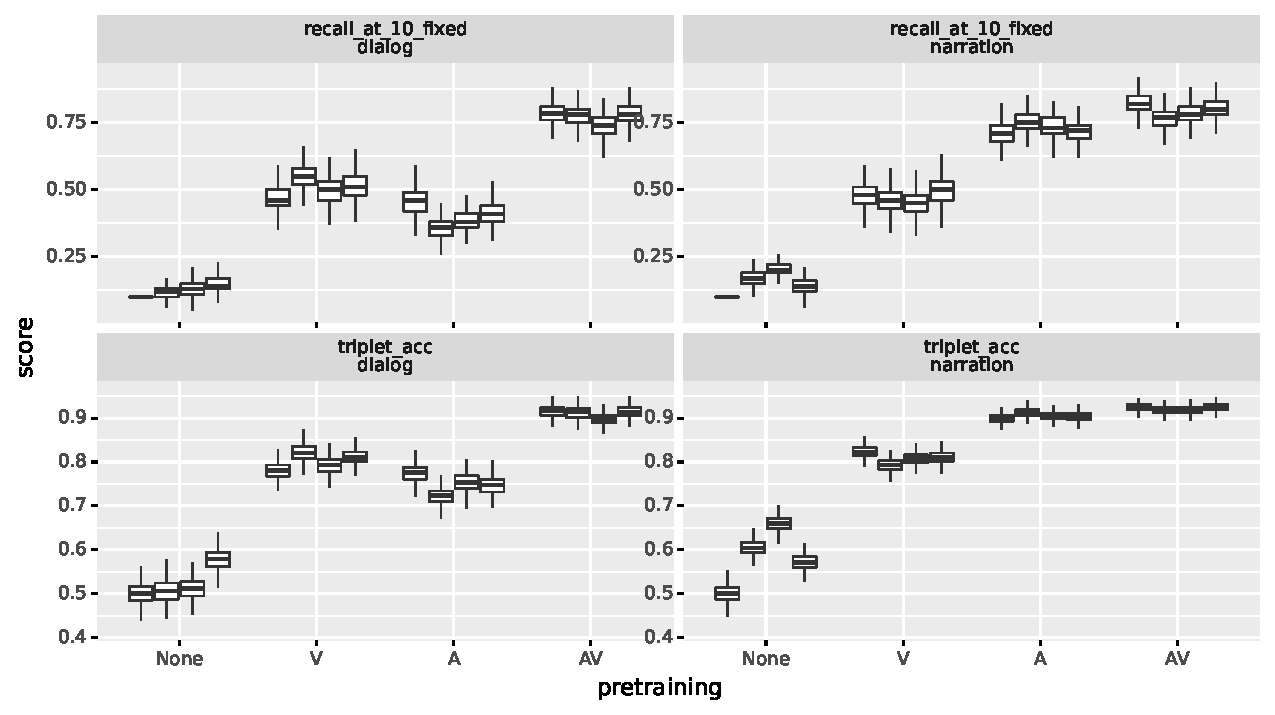
\includegraphics[width=\columnwidth]{results/ablations/pretraining.pdf}
	\caption{Effect of pre-training on performance on the dialog
          and narration validation data. The top row shows recall@10;
          the bottom row triplet accuracy.}
	\label{fig:pretraining}
      \end{figure}

The best overall performance on both the dialog and the narration data is 
achieved with a model where both the video and audio encoder are pre-trained 
before being fine-tuned on our data. The model with no pre-training in
either modality failed to converge and thus performs at random.


On narration data, for both metrics, we see a clear ranking of
configurations from best to worst: (AV) audio and video pre-training,
(A) audio pre-training, (V) video pre-training and (None) no
trainining. Meanwhile for dialog data, the performance between A and V
is comparable. In this absence of any pre-training (None) the model failed
to converge and therefore performs at chance level.\footnote{Some of
  the runs of this configuration did perform above chance but
  training is in general unstable.}

To further understand and disentangle the effects of audio pre-training and 
fine-tuning, we train a model with frozen parameters of the 
\textsc{wav2vec} module. The effect of this condition is show in \Cref{fig:freeze_wav2vec}.
\begin{figure}[htb]
  \centering
  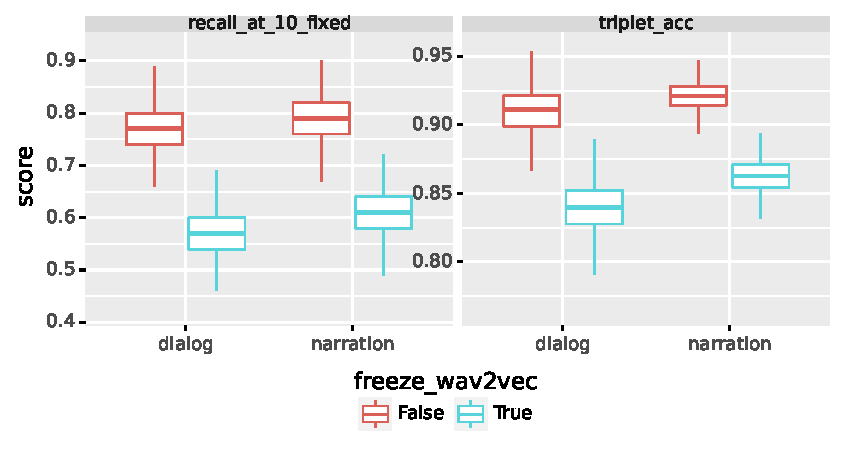
\includegraphics[width=\columnwidth]{results/ablations/freeze_wav2vec.pdf}
  \caption{Effect of freezing the parameters of the \textsc{wav2vec}
    module on model performance, on the dialog and narration
    validation data. The top row shows recall@10; the bottom row
    triplet accuracy.}
  \label{fig:freeze_wav2vec}
\end{figure}
We find without fine-tuning of the \textsc{wav2vec} module, performance decreases substantially 
on both metrics. In other words, best performance is only achieved with pre-trained and 
fine-tuned models.


\subsubsection{Jitter}
Next, we evaluate a model that has been trained with varying video and audio 
lengths (\textsc{jitter}). For fair comparison, we report recall@10 for both 
\textsc{fixed} and \textsc{jitter} validation configurations.
As seen in \Cref{fig:jitter}, the effect of \textsc{jitter} is only
minor and that performance is comparable.\footnote{However, we observe 
substantial performance improvements when using \textsc{jitter} in the more 
controlled minimal pairs evaluation (cf. \Cref{sec:minimal-pairs}))}
\begin{figure}[htb]
	\centering
	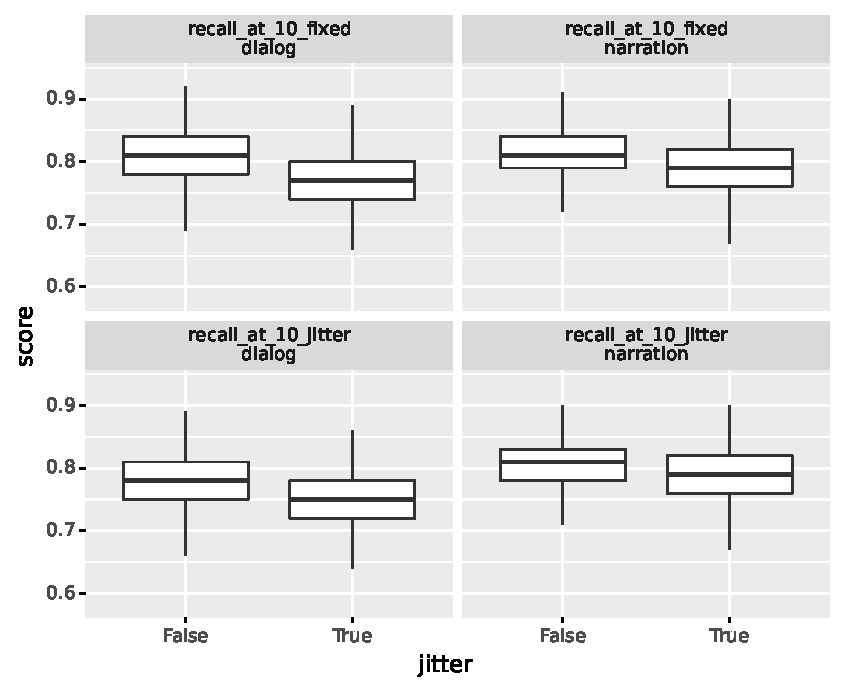
\includegraphics[width=\columnwidth]{results/ablations/jitter.pdf}
	\caption{Effect of jitter on model performance, on the dialog
          and narration validation data. The top row shows recall@10;
          the bottom row triplet accuracy.}
	\label{fig:jitter}
\end{figure}



\subsubsection{Temporal Information}
Finally, we explore the role of the temporal nature of the visual
modality.  \Cref{fig:static} compares the model with the regular video
encoder with one using the \textsc{static} baseline encoder.  For this
comparison we did not pre-train the video encoder in order to remove
the confound of the pre-training data.
Across
all metrics, we observe substantial performance drops for the
\textsc{static} model, which has access to the same video frames, but
does not leverage their temporal ordering. 
\begin{figure}[htb]
  \centering
  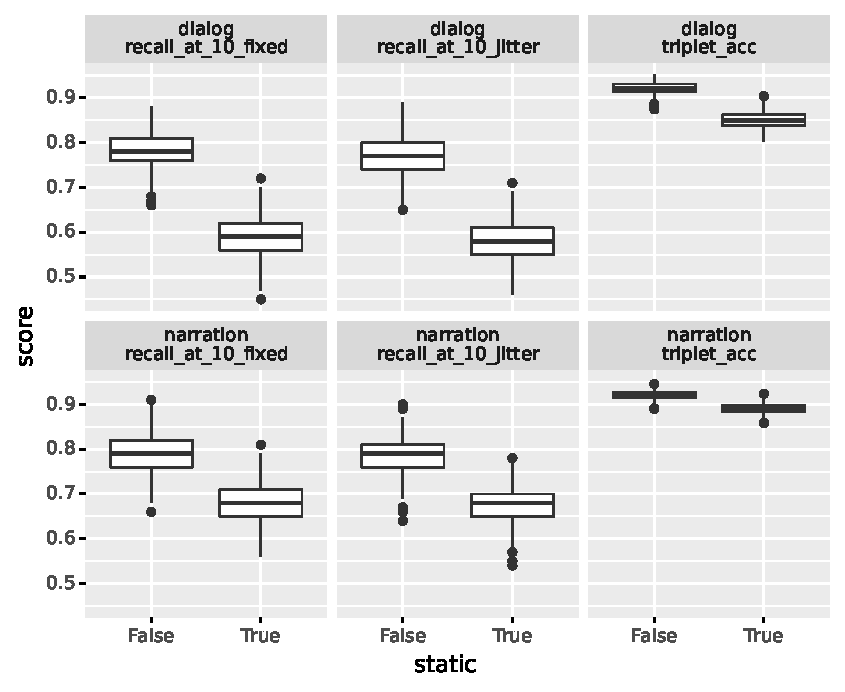
\includegraphics[width=\columnwidth]{results/ablations/static.pdf}
  \caption{Effect of a \textsc{static} image encoder on model performance, on 
  the dialog and narration validation data. The top row shows recall@10;
          the bottom row triplet accuracy.}
  \label{fig:static}
\end{figure}

\Cref{fig:scrambled_video} shows the effect of scrambling the video frames 
along the temporal dimension at test time. As expected, we observe substantial 
performance drops when the model does not see the video frames in 
the correct order.
\begin{figure}[htb]
	\centering
	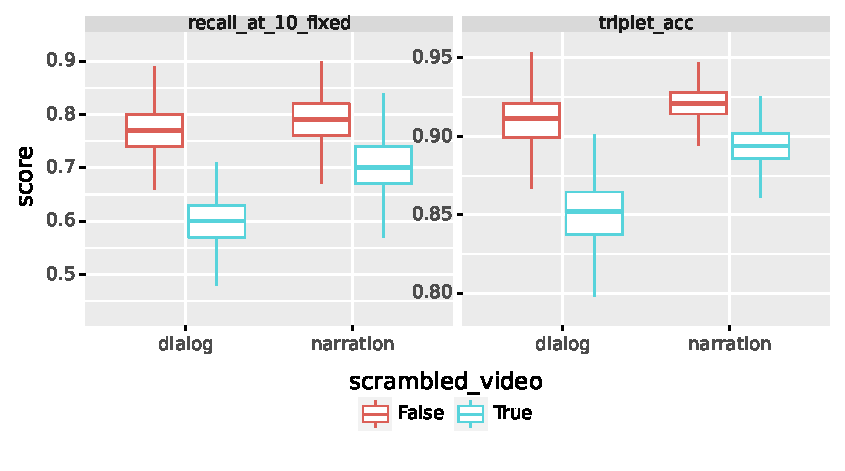
\includegraphics[width=\columnwidth]{results/ablations/scrambled_video.pdf}
	\caption{Effect of scrambling the video frames on model performance, on the 
	dialog and narration validation data. The top row shows recall@10;
		the bottom row triplet accuracy.}
	\label{fig:scrambled_video}
\end{figure}

\subsection{Minimal Pairs}
\label{sec:minimal-pairs}


\Cref{tab:minimal_pair_results} presents results for the minimal pair 
evaluation. We find that a models that are 
pre-trained and fine-tuned with \textsc{jitter} perform best. In the first two 
configurations, there is not much difference in the scores for verbs and nouns.

If the model is trained without \textsc{jitter}, performance for nouns drops 
substantially more than for verbs. For a model trained on \textsc{static} data, 
the performance for verbs is worse, confirming that temporal information is 
more important for the semantics 
of verbs.
\todo{MN: Add more rows regarding pre-training conditions?}
\todo{MN: Include standard deviation over 3 model runs}
\begin{table}[htb]
	\caption{Minimal pair accuracies for nouns and verbs for different model 
	configurations (Finet=Finetune \textsc{wav2vec} module; 
	Jitt=\textsc{jitter}; Tmp=Temporal information (not \textsc{static})). 
	Models have been pretrained on audio and video. Standard deviation 
	calculated using bootstrapping (100 re-samples).}
	\label{tab:minimal_pair_results}
	\begin{tabular}{lllll}
\toprule
     Finet &       Jitt &        Tmp &      Nouns &      Verbs \\
\midrule
\checkmark & \checkmark & \checkmark & 0.81±0.002 & 0.81±0.007 \\
           & \checkmark & \checkmark & 0.71±0.002 & 0.69±0.006 \\
\checkmark &            & \checkmark & 0.73±0.003 & 0.79±0.006 \\
\checkmark & \checkmark &            & 0.79±0.002 & 0.77±0.007 \\
\bottomrule
\end{tabular}

\end{table}

\Cref{fig:accuracy_targeted_triplets_nouns} and
\ref{fig:accuracy_targeted_triplets_verbs} show per-word
accuracy for nouns and verbs for the best performing model.
We perform bootstrapping (100 re-samples) to estimate mean and standard 
deviation for each accuracy score.


\begin{figure*}[htb]
  \centering
  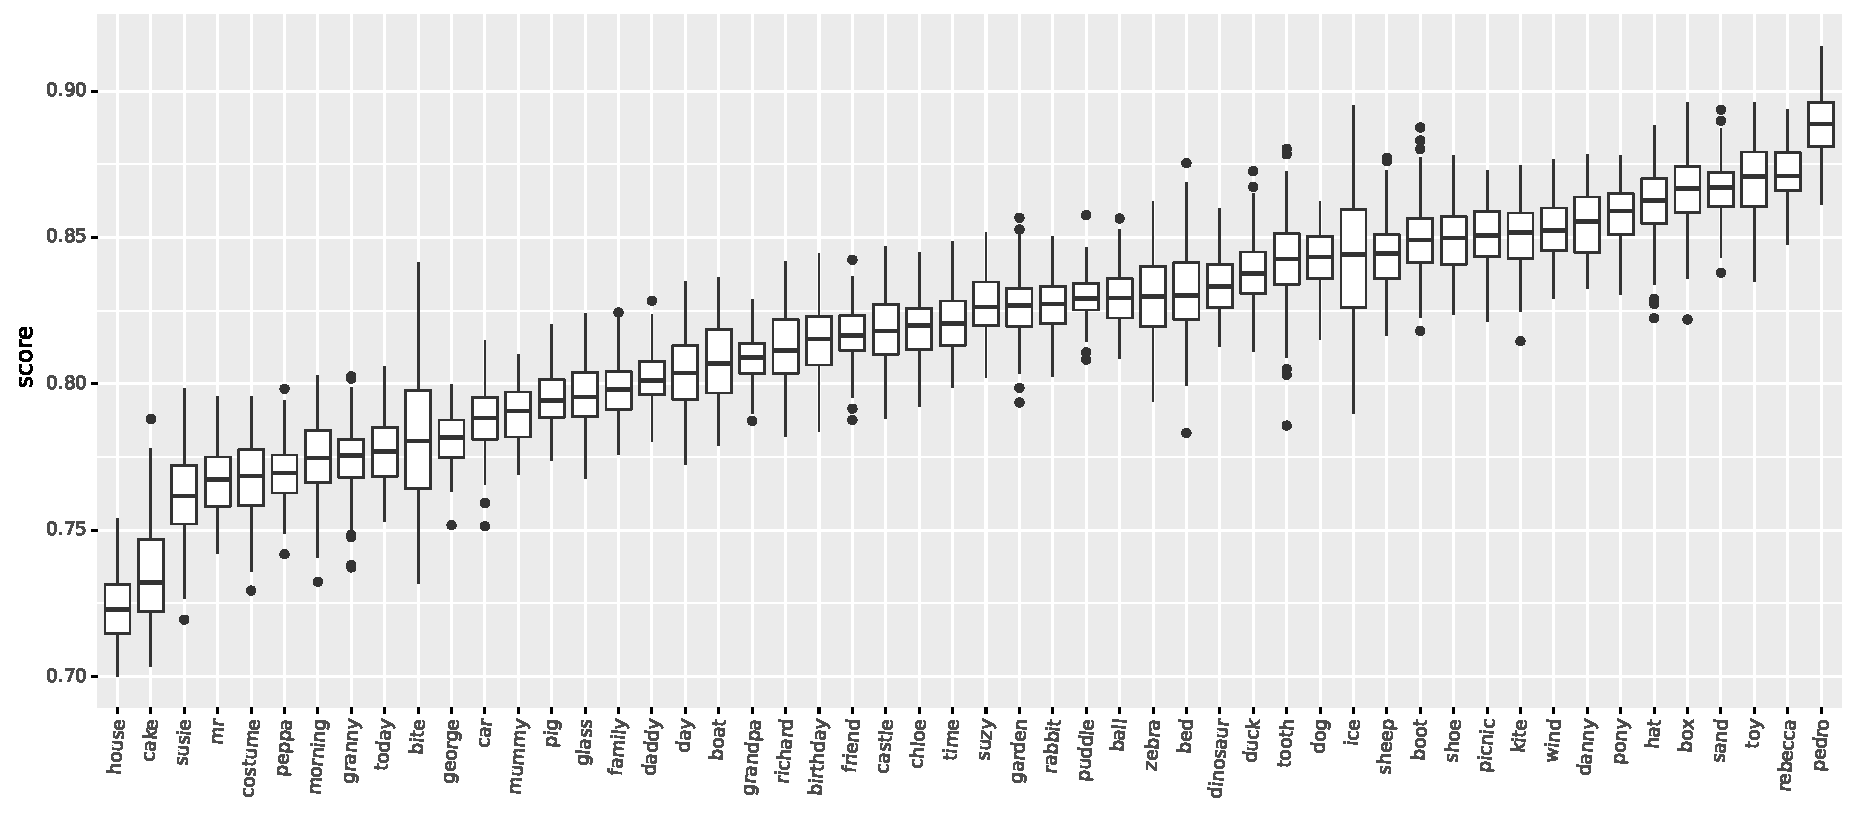
\includegraphics[width=\textwidth]{results/targeted_triplets/acc_per_word_NOUN.pdf}
  \caption{Per-word accuracies on the minimal pairs evaluation data for nouns.}
  \label{fig:accuracy_targeted_triplets_nouns}
\end{figure*}

\begin{figure}[htb]
  \centering
  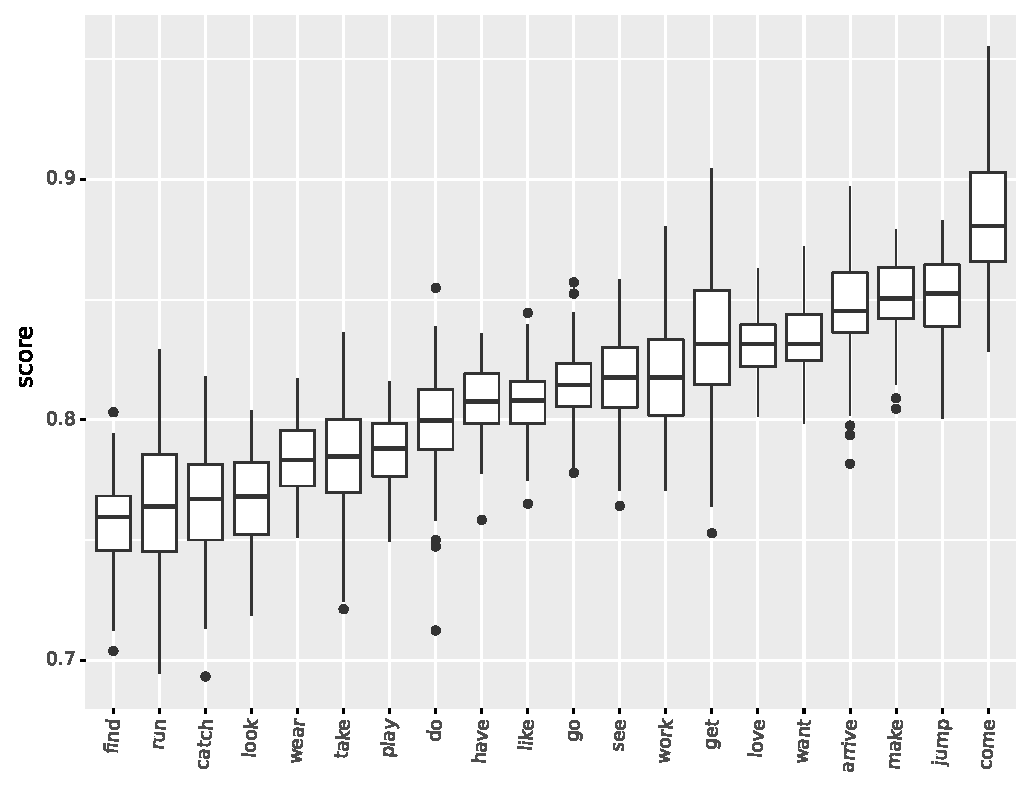
\includegraphics[width=\linewidth]{results/targeted_triplets/acc_per_word_VERB.pdf}
  \caption{Per-word accuracies on the minimal pairs evaluation data
    for verbs.}
  \label{fig:accuracy_targeted_triplets_verbs}
\end{figure}

We observe substantial variance in the accuracy scores, suggesting that the 
difficulty to learn certain words varies. For example, the 
scores for ``house'' and ``cake'' are very low. This could be because these 
concepts are not easy to ground, as they do not often refer to a similar visual 
entity. When looking at our evaluation examples, we find that indeed the word 
``house'' is used in varying visual contexts (house entrance, view of the whole 
house, inside the house, rabbit's house) and in displaced speech (talking about 
going to somebody's house). Regarding ``cake'', it refers to either a whole 
cake, a slice, dough, or crumbs.

On the other end, the words ``Pedro'' and ``Rebecca'' are learned very well: 
They refer to ``Pedro pony'' and ``Rebecca rabbit'', easily visually 
distinguishable from other characters which are mainly pigs. Additionally, they 
are usually central to the video scene when mentioned.

Further investigations with larger datasets are necessary to reveal the 
underlying reasons for difficulty, and relating them to predictors of age of 
acquisition in the child language acquisition literature 
\cite{roy2015predicting,frank2021variability}. 


